\documentclass[12pt]{article}
\usepackage{algos-tasks}

\begin{document}
\task[regular]{Marinara Trench}

\begin{question}
The Marinara Trench has recently been discovered! The trench starts at point 0 and extends for $n$ kilometres. Geologists have deduced a few features about it.
\begin{itemize}
    \item The trench has a single deepest point at some unknown point $d$ kilometres from point 0.
    \item The depth is 0 metres at the endpoints of the trench (i.e. at 0 and $n$ kilometres).
    \item The depth strictly increases from 0 to $d$ kilometres.
    \item The depth strictly decreases from $d$ to $n$ kilometres.
\end{itemize}

For example, it might look something like this:
\begin{center}
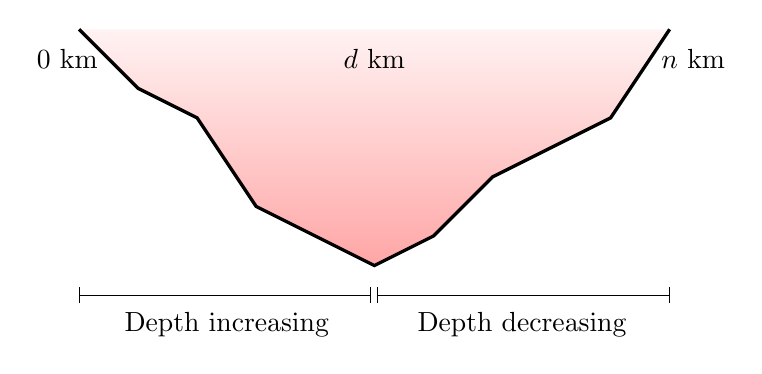
\begin{tikzpicture}[scale=0.75]
    \draw[draw=none, top color=red!5, bottom color=red!35]
        (0, 0) -- (1, -1) --  (2, -1.5) --  (3, -3) --  (4, -3.5) --  (5, -4) --  (6, -3.5) --  (7, -2.5) --  (8, -2) --  (9, -1.5) --  (10, -0) -- (0, 0);
    \draw[very thick]
        (0, 0) -- (1, -1) --  (2, -1.5) --  (3, -3) --  (4, -3.5) --  (5, -4) --  (6, -3.5) --  (7, -2.5) --  (8, -2) --  (9, -1.5) --  (10, -0);
    \node at (-0.2, -0.5) {$0$ km};
    \node at (10.4, -0.5) {$n$ km};
    \node at (5, -0.5) {$d$ km};
    \draw[|-|] (0, -4.5) -- (4.95, -4.5);
    \draw[|-|] (5.05, -4.5) -- (10, -4.5);
    \node at (2.5, -5) {Depth increasing};
    \node at (7.5, -5) {Depth decreasing};
\end{tikzpicture}
\end{center}

Scientists want to determine the position $d$ of the deepest point to within ten metres (0.01 kilometres). Note that the position of the deepest point is not the same as the depth of the deepest point! Unfortunately, since the trench is full of tomato sauce, measuring the depth at any particular point is very labour-intensive. Therefore, they want to use only a small number of measurements.

\begin{enumerate}
    \item Suppose that $n = 30$, i.e. the trench is 30 kilometres long. You have taken two measurements, so you know that at 10 km the depth is 600 metres, and at 20 km the depth is 800 metres. At which positions could the deepest point possibly be, and why?

    \textbf{Hint:} There are three regions to consider (and the boundary points between them). Given what we know about the trench, decide if it makes sense for the deepest point to lie within each region. Drawing a diagram might help!
    
    \item Now, we return to the general case, where the trench extends for $n$ kilometres (not necessarily 30km). By repeatedly applying the logic from part (a), we can find the deepest point in the trench to any precision we want. Design an algorithm based on part (a) to narrow the search range to within 0.01 kilometres. That is, your algorithm should find a range of points such that the deepest point is within this range, and the range covers no more than 0.01 kilometres.
    
    \item Use the Master Theorem to find an asymptotic bound on the number of measurements required using this method.
\end{enumerate}
\end{question}

\begin{rubric}
\begin{enumerate}
    \item Identify which range of positions could be the deepest point of the trench. Briefly explain why any other points cannot be the deepest.
    \item Give an algorithm that uses the logic of part (a) to determine the position of the deepest point. Your algorithm should find a range no more than 0.01 kilometres wide that contains the deepest point $d$.
    \item Apply the Master Theorem to determine asymptotically the number of measurements required. You must include the recurrence and which case of the theorem that applies.    
\end{enumerate}
Expected response length: a short paragraph for (a) and (c), a paragraph for (b).
\end{rubric}

\begin{solution}
\end{solution}

\begin{attribution}
\end{attribution}

\end{document}